\documentclass[11pt,a4j]{jsarticle}
\usepackage{float,array,booktabs,here}
\usepackage{amsmath}
\usepackage{bm}
\usepackage[dvipdfmx]{graphicx}
% \usepackage[whole]{bxcjkjatype}%日本語もコンパイル可にする.
%\usepackage[dvipdfmx,hiresbb]{graphicx}
\usepackage[top=25truemm,bottom=25truemm,left=25truemm,right=25truemm]{geometry}

\title{Computer Vision}
\author{81819433 開放環境科学専攻情報工学専修 修士1年 飯塚 健介}
\date{\today}
\begin{document}
    \maketitle

    \section{section name}
    \subsection{subsection name}

    \section{目的と課題設定}
    授業と関連した内容についてのレポートということで、
    私は主にセグメンテーションについて理解を深めるために授業で習った手法を用いてセグメンテーションの処理を自分で実装して
    OpenCVに備わっているライブラリ関数での実装と検討、また自分の実装について考察を行う。


    \section{開発及び実行環境}
    開発及び実行環境は次のとおりである。OpenCVは比較と入出力を受け取るために利用した。
    \begin{itemize}
        \item OS : Ubuntu18.04 
        \item 使用言語 : Python3.6.5, C++11 
        \item 使用ライブラリ : Numpy, Matplotlib, OpenCV 
       \end{itemize}

    \section{k-means法を用いたセグメンテーション}
    まず、k-means法を用いたセグメンテーションについて検討と実装を行った。

    \subsection{k-means法について}
    \cite{k-means}を参考にアルゴリズムについて検討した。k-meansではいくつのクラスタに分類するかを人が指定しなければいけない。
    そしてランダムにクラスタリングされた次元のベクトルについて各クラスタの重心を求める。その重心から各ベクトルのユークリッド距離を算出し
    最小となるクラスタに属するようにする。これをクラスタリング結果が前回のクラスタリング結果と一致するまでもしくはある上限回数行い、各クラスタの重心を決定する。
    ここに新たな入力ベクトルが入ってきた場合には各クラスタの重心とのユークリッド距離を算出し最小となったクラスタに属するようにする。
    \subsection{実装方法}
    \subsection{結果と考察}

    \section{mean-shiftを用いたセグメンテーション}
    \subsection{mean-shiftについて}
    \subsection{実装方法}
    \subsection{結果と考察}

    \section{結論とまとめ}

    \begin{thebibliography}{9}
        \bibitem{k-means} http://home.deib.polimi.it/matteucc/Clustering/tutorial_html/kmeans.html
        \bibitem{susan} S. M. Smith and J. M. Brady,
          ``SUSAN|A new approach to low level image processing,'' Int. J. Comput.
          Vis., vol.23, no.1, pp.45-78, May 1997.
      \end{thebibliography}

    \begin{figure}[H]
      \centering
      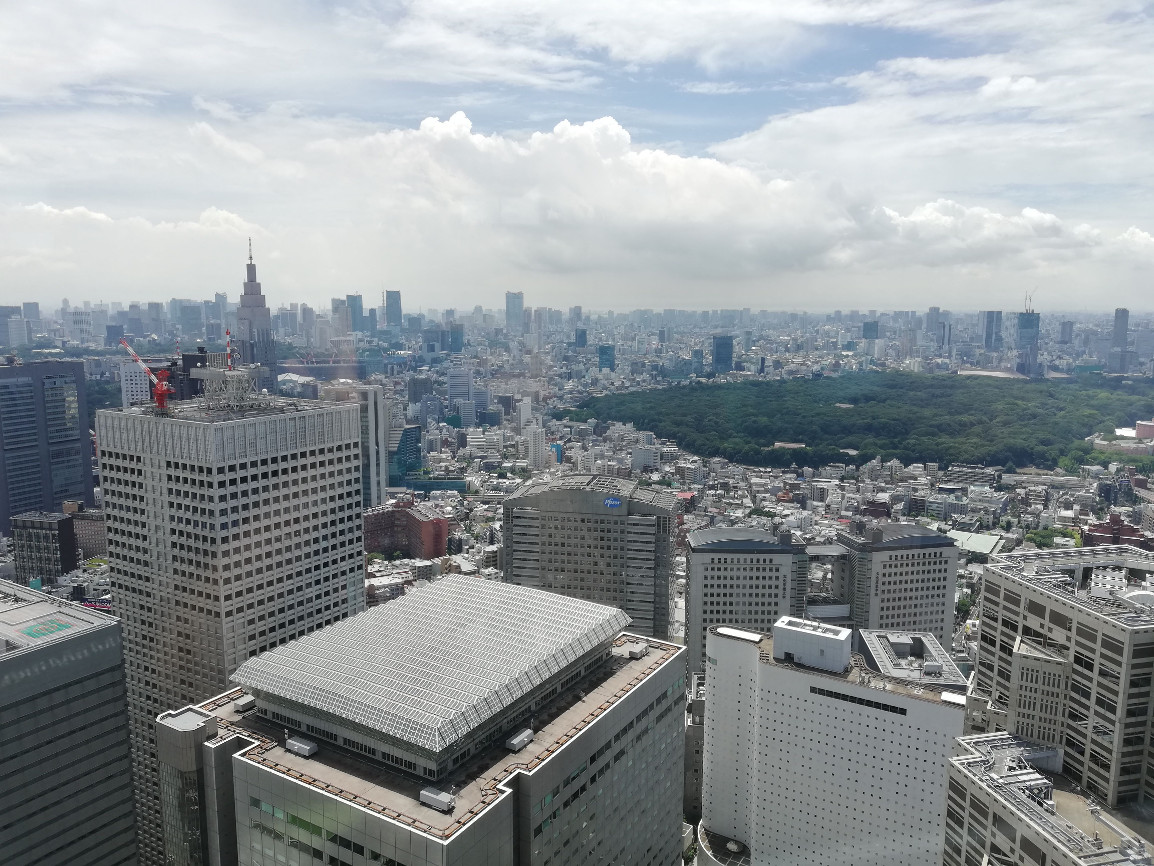
\includegraphics[clip,width=4.0cm]{img/metro.jpg}
      \caption{都庁南展望台からの写真\label{fig:cute}}
    \end{figure}

    \begin{equation}
        s\left(
        \begin{array}{c}
            u \\
            v \\
            1
        \end{array}
        \right) =
        \left(
    \begin{array}{cccc}
      P_{11} & P_{12} & P_{13} & P_{14}\\
      P_{21} & P_{22} & P_{23} & P_{24} \\
      P_{31} & P_{32} & P_{33} & P_{34} \\
    \end{array}
        \right)
        \left(
        \begin{array}{c}
            X \\
            Y \\
            Z \\
            1
        \end{array}
        \right)
        \label{eq:projection_matrix}
    \end{equation}

\end{document}
